% Titre de la premiere partie

\section{Introduction au système : DPI}
%%%%%%%%%%%%%%%%%%%%%%%%%%%%%%%%%%%%%%%%%%%%%%%%
% Première diapo
%%%%%%%%%%%%%%%%%%%%%%%%%%%%%%%%%%%%%%%%%%%%%%%%
\begin{frame}
\frametitle{Introduction au système : DPI}
\framesubtitle{Problème}

\begin{itemize}
	\item	<1->	Le contrôle d'accès aux espaces privés.
	%\item	<2->	Contraintes : Luminosité, Bruit, Angle d'inclinaison ...
\end{itemize}

\begin{figure}
\begin{overprint}
	\onslide<1>\centering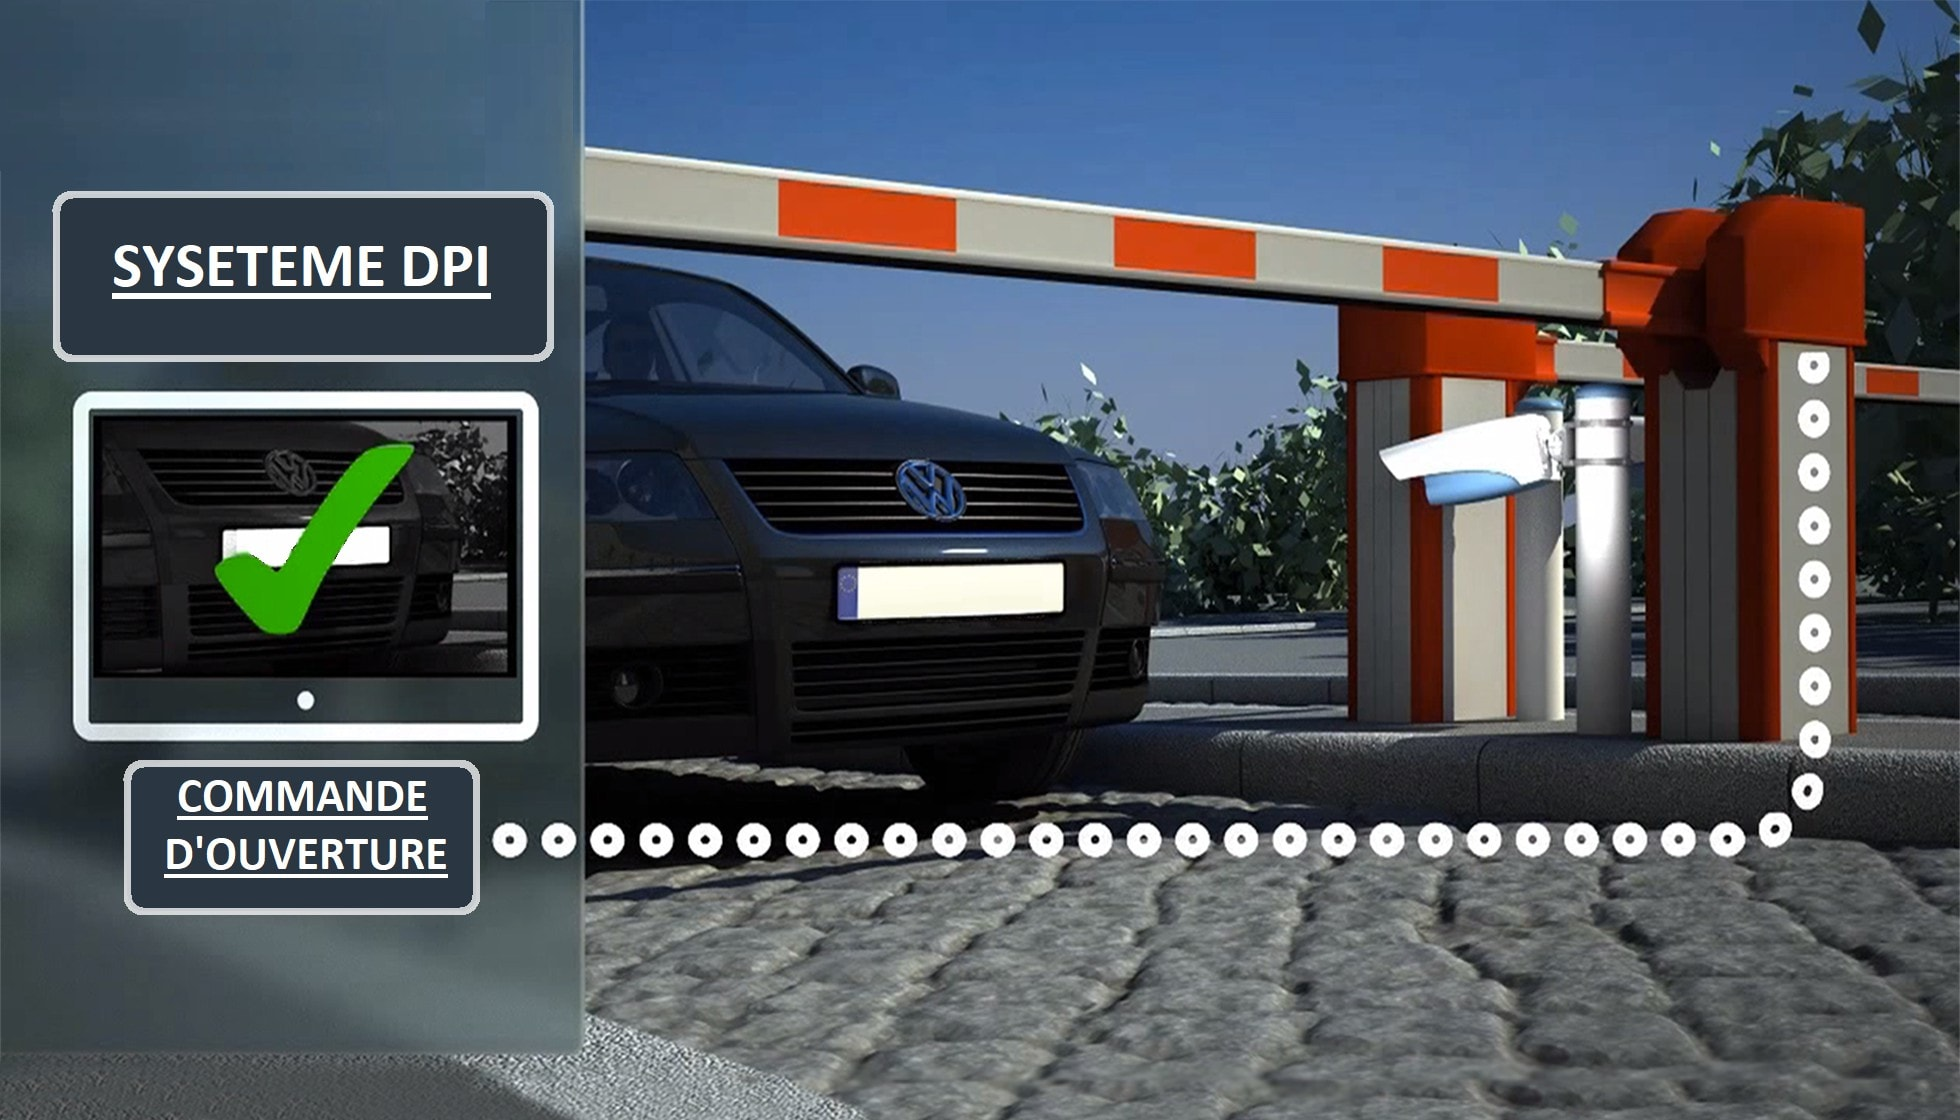
\includegraphics[width=0.7\linewidth]{figures/DPI.PNG}\caption{Exemple d'application du système}
	%\onslide<2>\centering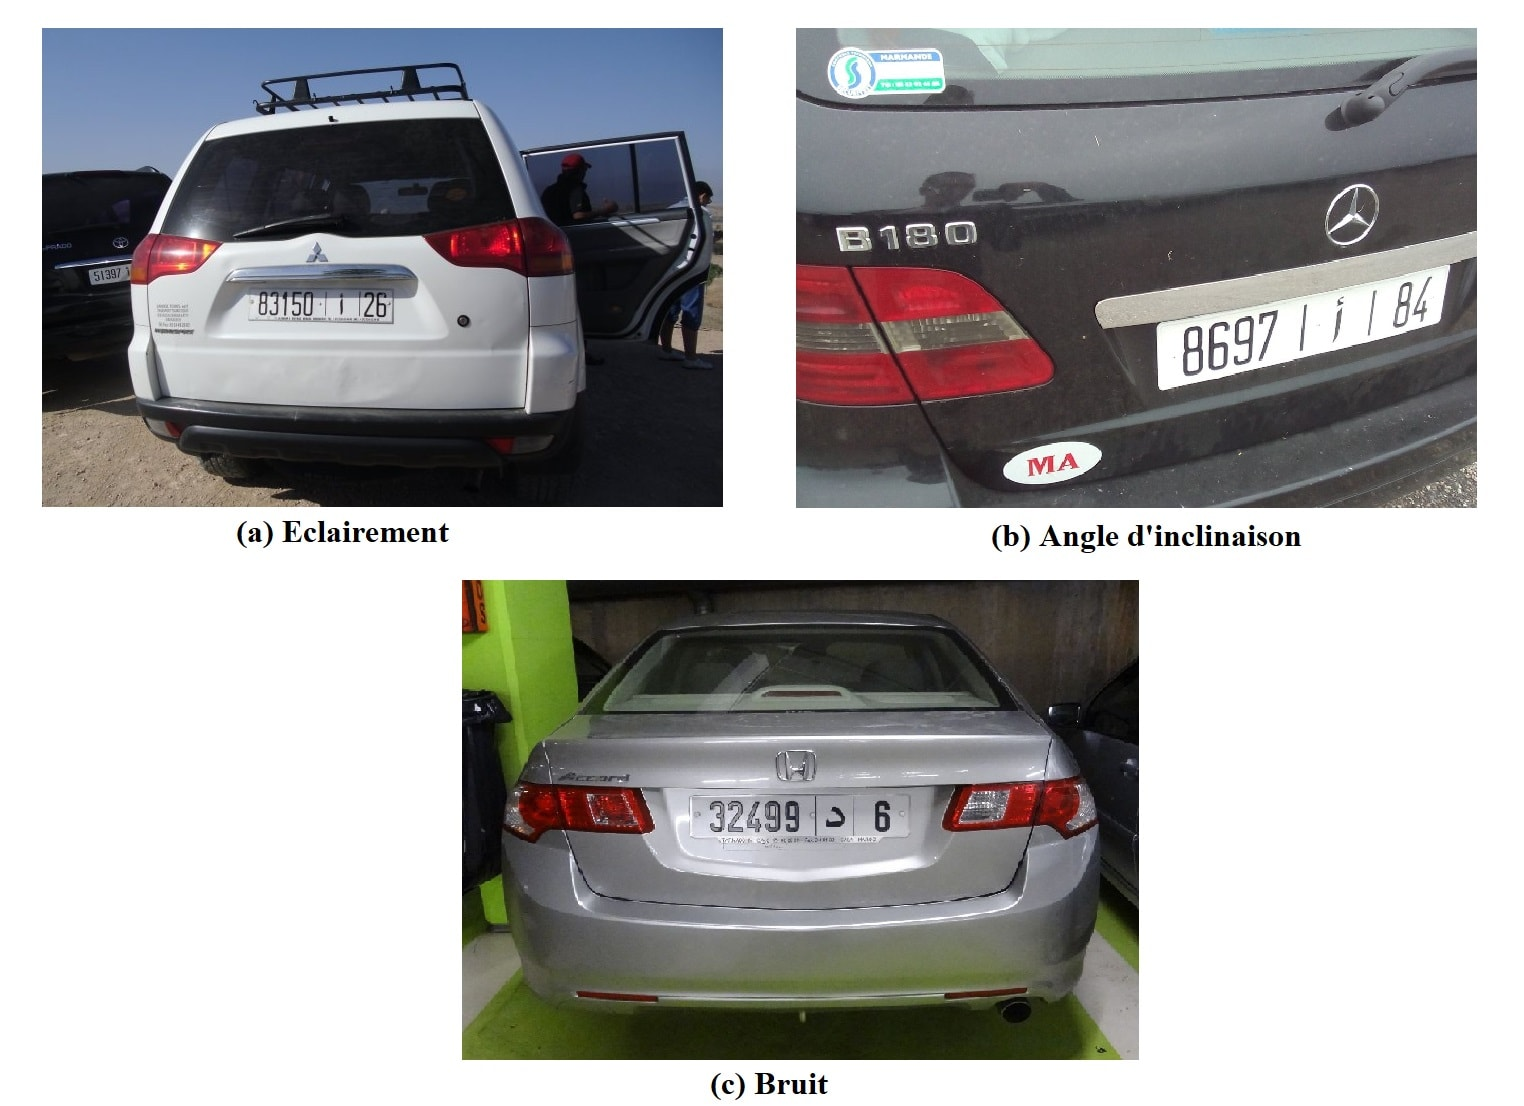
\includegraphics[width=0.6\linewidth]{figures/Contraintes.PNG}\caption{Contraintes de détection}
\end{overprint}
\end{figure}
	
\end{frame}


%%%%%%%%%%%%%%%%%%%%%%%%%%%%%%%%%%%%%%%%%%%%%%%%
% Troisième diapo
%%%%%%%%%%%%%%%%%%%%%%%%%%%%%%%%%%%%%%%%%%%%%%%%
\begin{frame}
\frametitle{Introduction au système : DPI}
\framesubtitle{Solution}

\begin{itemize}
	\item	<1>	Un processus simple et dynamique assurant une detection rapide et précise des plaques !
	\begin{figure}
	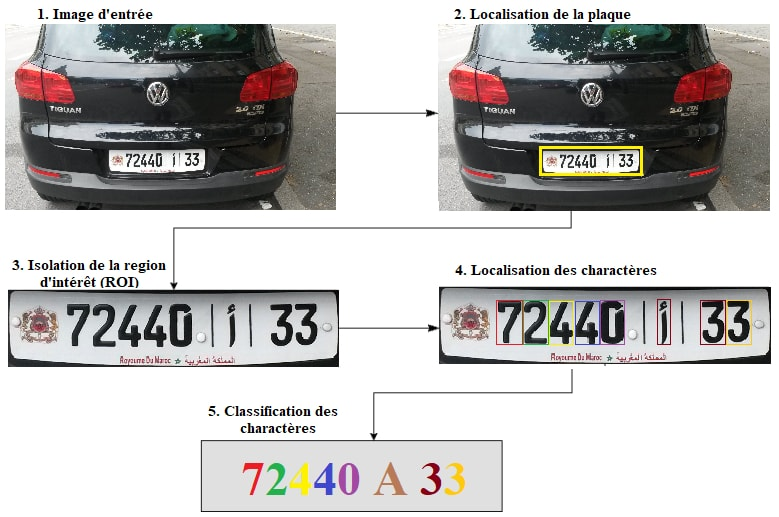
\includegraphics[width=0.7\linewidth]{figures/Process.PNG}\caption{Le processus de reconnaissance optimal}
	\end{figure}
\end{itemize}

\end{frame}

%%%%%%%%%%%%%%%%%%%%%%%%%%%%%%%%%%%%%%%%%%%%%%%%
% Deuxième diapo
%%%%%%%%%%%%%%%%%%%%%%%%%%%%%%%%%%%%%%%%%%%%%%%%
\begin{frame}
\frametitle{Introduction au système : DPI}
\framesubtitle{Analyse Fonctionnelle}
\captionsetup{justification=centering}

\begin{figure}
    \centering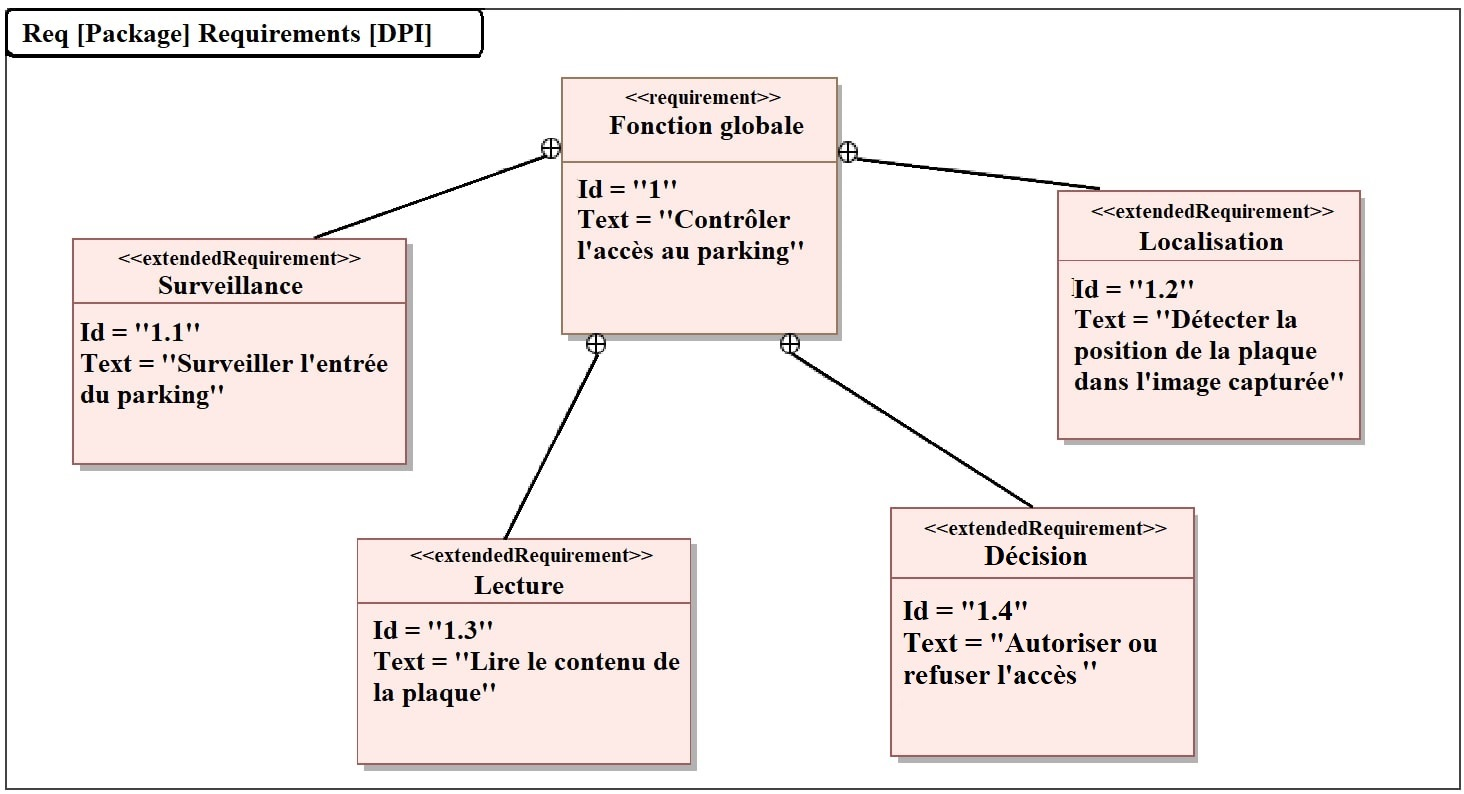
\includegraphics[width=0.9\linewidth]{figures/Req.PNG}\caption{Diagramme d'exigences}
\end{figure}
\end{frame}
%%%%%%%%%%%%%%%%%%%%%%%%%%%%%%%%%%%%%%%%%%%%%%%%
% Quatième diapo
%%%%%%%%%%%%%%%%%%%%%%%%%%%%%%%%%%%%%%%%%%%%%%%%
\begin{frame}
\frametitle{Introduction au système : DPI}
\framesubtitle{Une approche}

\begin{itemize}
    \item	<1>    Développer des algorithmes basés sur les nouvelles techniques d'apprentissage profond pour la localisation et la reconnaissance.
\end{itemize}
\begin{figure}
    
\includegraphics[width=1\linewidth]{figures/Biblio.PNG}\caption{Les trois bibliothèques essentielles}
\end{figure}
        
\end{frame}